\PassOptionsToPackage{unicode=true}{hyperref} % options for packages loaded elsewhere
\PassOptionsToPackage{hyphens}{url}
%
\documentclass[ignorenonframetext,aspectratio=169,ignorenonframetext]{beamer}
\usepackage{pgfpages}
\setbeamertemplate{caption}[numbered]
\setbeamertemplate{caption label separator}{: }
\setbeamercolor{caption name}{fg=normal text.fg}
\beamertemplatenavigationsymbolsempty
% Prevent slide breaks in the middle of a paragraph:
\widowpenalties 1 10000
\raggedbottom
\setbeamertemplate{part page}{
\centering
\begin{beamercolorbox}[sep=16pt,center]{part title}
  \usebeamerfont{part title}\insertpart\par
\end{beamercolorbox}
}
\setbeamertemplate{section page}{
\centering
\begin{beamercolorbox}[sep=12pt,center]{part title}
  \usebeamerfont{section title}\insertsection\par
\end{beamercolorbox}
}
\setbeamertemplate{subsection page}{
\centering
\begin{beamercolorbox}[sep=8pt,center]{part title}
  \usebeamerfont{subsection title}\insertsubsection\par
\end{beamercolorbox}
}
\AtBeginPart{
  \frame{\partpage}
}
\AtBeginSection{
  \ifbibliography
  \else
    \frame{\sectionpage}
  \fi
}
\AtBeginSubsection{
  \frame{\subsectionpage}
}
\usepackage{lmodern}
\usepackage{amssymb,amsmath}
\usepackage{ifxetex,ifluatex}
\usepackage{fixltx2e} % provides \textsubscript
\ifnum 0\ifxetex 1\fi\ifluatex 1\fi=0 % if pdftex
  \usepackage[T1]{fontenc}
  \usepackage[utf8]{inputenc}
  \usepackage{textcomp} % provides euro and other symbols
\else % if luatex or xelatex
  \usepackage{unicode-math}
  \defaultfontfeatures{Ligatures=TeX,Scale=MatchLowercase}
\fi
% use upquote if available, for straight quotes in verbatim environments
\IfFileExists{upquote.sty}{\usepackage{upquote}}{}
% use microtype if available
\IfFileExists{microtype.sty}{%
\usepackage[]{microtype}
\UseMicrotypeSet[protrusion]{basicmath} % disable protrusion for tt fonts
}{}
\IfFileExists{parskip.sty}{%
\usepackage{parskip}
}{% else
\setlength{\parindent}{0pt}
\setlength{\parskip}{6pt plus 2pt minus 1pt}
}
\usepackage{hyperref}
\hypersetup{
            pdftitle={OS EFEITOS DOS COMPONENTES DO SPREAD EX-POST NA RENTABILIDADE DAS INSTITUIÇÕES BANCÁRIAS},
            pdfauthor={JACKSON DA SILVA TORRES},
            pdfborder={0 0 0},
            breaklinks=true}
\urlstyle{same}  % don't use monospace font for urls
\newif\ifbibliography
\usepackage{longtable,booktabs}
\usepackage{caption}
% These lines are needed to make table captions work with longtable:
\makeatletter
\def\fnum@table{\tablename~\thetable}
\makeatother
\setlength{\emergencystretch}{3em}  % prevent overfull lines
\providecommand{\tightlist}{%
  \setlength{\itemsep}{0pt}\setlength{\parskip}{0pt}}
\setcounter{secnumdepth}{0}

% set default figure placement to htbp
\makeatletter
\def\fps@figure{htbp}
\makeatother

\usepackage[utf8]{inputenc} % codificacao de caracteres
\usepackage[T1]{fontenc}    % codificacao de fontes
\usepackage[brazil]{babel}  % idioma
\usepackage{graphicx}       %fundo
\usetheme{default}          % tema
\usecolortheme{orchid}     % cores
\usefonttheme[onlymath]{serif} % fonte modo matematico
\usepackage{wallpaper}

\usepackage{tikz}

\usepackage[
style=abnt,
backref=true,
backend=biber,
maxcitenames=2,
%citecounter=true,
backrefstyle=three,
%nohashothers=true
]{biblatex}

%\setbeameroption{show notes}
%\setbeameroption{show notes on second screen=right}

%\usepackage[pdftex]{graphicx}

\usepackage[final]{pdfpages}

\usepackage{booktabs}

\usepackage{helvet}
\renewcommand{\familydefault}{\sfdefault}
\makeindex
\DeclareUnicodeCharacter{0301}{******}
\DeclareUnicodeCharacter{0303}{******}
\DeclareUnicodeCharacter{0327}{******}
\DeclareUnicodeCharacter{0302}{******}

\title{OS EFEITOS DOS COMPONENTES DO \emph{SPREAD} \emph{EX-POST} NA
RENTABILIDADE DAS INSTITUIÇÕES BANCÁRIAS}
\author{JACKSON DA SILVA TORRES}
\date{2021}

\begin{document}
\frame{\titlepage}

\begin{frame}{\textbf{SUMÁRIO }}
\protect\hypertarget{sumuxe1rio}{}

\begin{columns}[T]
\begin{column}{0.6\textwidth}
\begin{enumerate}
\item
  \textbf{INTRODUÇÃO}

  \begin{enumerate}
  \item
    CONTEXTUALIZAÇÃO
  \item
    OBJETIVOS
  \item
    JUSTIFICATIVA TEÓRICA E PRÁTICA
  \item
    ESTRUTURA DA DISSERTAÇÃO
  \end{enumerate}
\item
  \textbf{REFERENCIAL TEÓRICO}

  \begin{enumerate}
  \item
    SETOR BANCÁRIO NO BRASIL
  \item
    SPREAD BANCÁRIO
  \item
    ESTUDOS ANTERIORES
  \end{enumerate}
\end{enumerate}
\end{column}

\begin{column}{0.4\textwidth}
\begin{enumerate}
\setcounter{enumi}{2}
\tightlist
\item
  \textbf{PROCEDIMENTOS METODOLÓGICOS}
\end{enumerate}
\end{column}
\end{columns}

\end{frame}

\begin{frame}{\textbf{1.1 CONTEXTUALIZAÇÃO}}
\protect\hypertarget{contextualizauxe7uxe3o}{}

\begin{enumerate}
[a.]
\item
  \textbf{Spread} como indicador de \textbf{desempenho da economia}
  (BANK and IMF \protect\hyperlink{ref-WB:2005}{2005}; Levine
  \protect\hyperlink{ref-levine:1997}{1997}; Dantas
  \protect\hyperlink{ref-dantas:2012}{2012}; Leal
  \protect\hyperlink{ref-leal:2006}{2006})

  \begin{itemize}
  \item
    \textbf{Elevados níveis} de \textbf{Spread} atuam no
    \textbf{desfavorecimento do crédito}.
  \item
    Fundo Monetário Internacional (FMI) e Banco Mundial (BM) realizam e
    incentivam estudos sobre o indicador a nível mundial {[}BANK and IMF
    (\protect\hyperlink{ref-WB:2005}{2005}).

    \begin{itemize}
    \tightlist
    \item
      A maioria indica a \textbf{relação inversa} entre \textbf{Spread}
      e \textbf{desenvolvimento econômico}
    \end{itemize}
  \end{itemize}
\item
  \textbf{Spread} como \textbf{indicador de eficência} do
  \textbf{Sistema Financeiro}\\
  (Levine \protect\hyperlink{ref-levine:1997}{1997}; Dantas
  \protect\hyperlink{ref-dantas:2012}{2012}; Leal
  \protect\hyperlink{ref-leal:2006}{2006})

  \begin{itemize}
  \tightlist
  \item
    Relacionado com a \textbf{solidez} e \textbf{competitividade} das
    instituições
  \end{itemize}
\end{enumerate}

\textcolor{blue}{DESENVOLVIMENTO ECONÔMICO X SISTEMA FINANCEIRO SÓLIDO}

\end{frame}

\begin{frame}{\textbf{1.2 OBJETIVOS}}
\protect\hypertarget{objetivos}{}

\textbf{OBJETIVO GERAL}

\begin{enumerate}
\tightlist
\item
  \textbf{Verificar} quais \textbf{variáveis} microeconômicas e
  macroeconômicas exercem \textbf{influência significativa} sobre o
  \textbf{spread ex-post} e como estas \textbf{afetam} a
  \textbf{rentabilidade} das \textbf{instituições bancárias}
  brasileiras.
\end{enumerate}

\textcolor{blue}{PONTO ÓTIMO QUE MAXIMIZA OS LUCROS E MINIMIZA O CUSTO DE CRÉDITO}

\end{frame}

\begin{frame}{\textbf{1.2 OBJETIVOS}}
\protect\hypertarget{objetivos-1}{}

\textbf{OBJETIVOS ESPECÍFICOS}

\begin{enumerate}
\item
  Realizar \textbf{levantamento teórico e bibliográfico} sobre
  \textbf{setor bancário} e estudos sobre o \textbf{Spread} bancário no
  Brasil;
\item
  \textbf{Identificar} e \textbf{testar} \textbf{variáveis}
  macroeconômicas e microeconômicas enquanto \textbf{componentes}
  \textbf{determinantes} do \textbf{spread} bancário \emph{ex-post};
\item
  \textbf{Analisar} e \textbf{estimar} como as \textbf{variações dos
  componentes do \emph{spread}} bancário \textbf{afetam} a
  \textbf{rentabilidade} dos \textbf{bancos}.
\end{enumerate}

\end{frame}

\begin{frame}{\textbf{1.3 JUSTIFICATIVA TEÓRICA E PRÁTICA}}
\protect\hypertarget{justificativa-teuxf3rica-e-pruxe1tica}{}

\begin{itemize}
\item
  \textbf{Evidências} da \textbf{influência} do nível de \textbf{Spread}
  no desenvolvimento econômico.
\item
  \textbf{Importância} do \textbf{Spread} na \textbf{solidez} do
  \textbf{sistema financeiro}.
\item
  \textbf{Economia} e \textbf{Mercado Financeiro} em \textbf{constantes
  transformações}.
\item
  O \textbf{cenário brasileiro} é \textbf{considerado peculiar} por
  possuir histórico de (Levine
  \protect\hyperlink{ref-levine:1997}{1997}; Matos
  \protect\hyperlink{ref-matos:2003}{2003}):

  \begin{itemize}
  \item
    \textbf{Elevados níveis} de \textbf{spread} bancário
  \item
    \textbf{Baixa relação} entre \textbf{crédito e PIB}
  \item
    \textbf{Cenários} de \textbf{crescimento econômico}
    \textbf{instáveis} e considerados \textbf{baixos}
  \end{itemize}
\item
  \textbf{Carências} de \textbf{pesquisas} acerca do
  \textbf{\emph{Spread ex-post}}
\item
  Existência de lacunas, divergências e incogluências de pesquisas.
\end{itemize}

\end{frame}

\begin{frame}{\textbf{2.1 SETOR BANCÁRIO NO BRASIL}}
\protect\hypertarget{setor-bancuxe1rio-no-brasil}{}

\begin{columns}[T]
\begin{column}{0.5\textwidth}
\begin{itemize}
\item
  \textbf{Contexto Histórico}
\item
  \textbf{Evolução}
\item
  \textbf{Organização}

  \begin{itemize}
  \tightlist
  \item
    Sistema Financeiro Nacional
  \item
    Órgãos Normativos
  \item
    Órgão Supervisores
  \item
    Operadores

    \begin{itemize}
    \tightlist
    \item
      Bancos e Caixas Econômicas
    \item
      Banco Comercial
    \item
      Banco de Investimento
    \item
      Banco de Desenvolvimento
    \item
      Banco de Câmbio
    \item
      Banco Múltiplos
    \item
      Caixa Econômica
    \end{itemize}
  \end{itemize}
\end{itemize}
\end{column}

\begin{column}{0.5\textwidth}
\begin{itemize}
\tightlist
\item
  \textbf{Características}

  \begin{itemize}
  \tightlist
  \item
    Concentração Bancária
  \item
    Tendência para domínio da participação estrangeira
  \item
    Elevados níveis de \emph{Spread} bancário
  \item
    Histórico de baixa relação Crédito/PIB
  \item
    Histórico de crescimento instável
  \end{itemize}
\end{itemize}
\end{column}
\end{columns}

\end{frame}

\begin{frame}{\textbf{2.1 SETOR BANCÁRIO NO BRASIL}}
\protect\hypertarget{setor-bancuxe1rio-no-brasil-1}{}

\textbf{EVOLUÇÃO DE DADOS}

\begin{columns}[T]
\begin{column}{0.33333\textwidth}
\begin{center}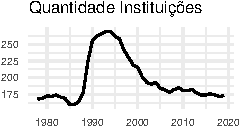
\includegraphics{01-presentation-V1_files/figure-beamer/count.banks-1} \end{center}

\begin{center}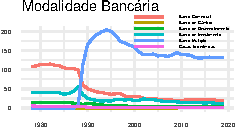
\includegraphics{01-presentation-V1_files/figure-beamer/kind.banks-1} \end{center}
\end{column}

\begin{column}{0.33333\textwidth}
\begin{center}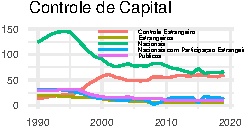
\includegraphics{01-presentation-V1_files/figure-beamer/control.banks-1} \end{center}

\begin{center}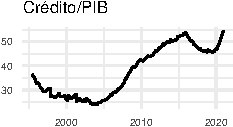
\includegraphics{01-presentation-V1_files/figure-beamer/credit.pib-1} \end{center}
\end{column}

\begin{column}{0.33333\textwidth}
\begin{center}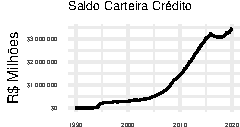
\includegraphics{01-presentation-V1_files/figure-beamer/credit balance-1} \end{center}

\begin{center}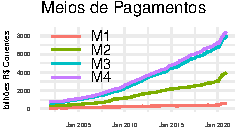
\includegraphics{01-presentation-V1_files/figure-beamer/mpplot-1} \end{center}
\end{column}
\end{columns}

\end{frame}

\begin{frame}{\textbf{2.2 SPREAD BANCÁRIO}}
\protect\hypertarget{spread-bancuxe1rio}{}

\begin{itemize}
\tightlist
\item
  \textbf{CONCEITOS}

  \begin{itemize}
  \tightlist
  \item
    O termo \emph{spread} significa --- tradução livre ---
    \textbf{amplitude}, \textbf{crescimento} e \textbf{extensão}.
  \item
    Utilizado no \textbf{setor financeiro} no sentido de \textbf{margem}
  \item
    É obtido através da \textbf{diferença} entre a \textbf{taxa de
    aplicação} e a \textbf{taxa de captação}

    \begin{itemize}
    \tightlist
    \item
      Diferença entre custos operacionais (BACEN
      \protect\hyperlink{ref-BCB:2016}{2016}) (BACEN
      \protect\hyperlink{ref-BCB:2000}{2000}).
    \end{itemize}
  \end{itemize}
\end{itemize}

\[
\textbf{Spread} = \textbf{Taxa de Aplicação} - \textbf{Taxa de Captação}
\]

\begin{itemize}
\tightlist
\item
  O \textbf{spread} bancário representa uma medida que sinaliza o
  desempenho dos bancos (Levine
  \protect\hyperlink{ref-levine:1997}{1997}) e indicador de eficiência
  da economia(BANK and IMF \protect\hyperlink{ref-WB:2005}{2005}).
\end{itemize}

\end{frame}

\begin{frame}{\textbf{2.2 SPREAD BANCÁRIO}}
\protect\hypertarget{spread-bancuxe1rio-1}{}

\begin{columns}[T]
\begin{column}{0.5\textwidth}
\textbf{ÓTICAS} (Dick \protect\hyperlink{ref-dick:1999}{1999})

\begin{center}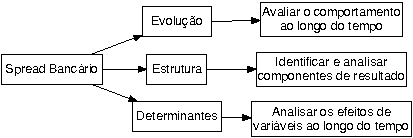
\includegraphics{01-presentation-V1_files/figure-beamer/diagram.otic-1} \end{center}
\end{column}

\begin{column}{0.5\textwidth}
\textbf{CARACTERÍSTICAS} (Leal \protect\hyperlink{ref-leal:2006}{2006})

\begin{center}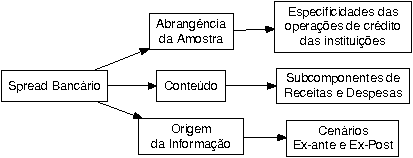
\includegraphics{01-presentation-V1_files/figure-beamer/diagram.carac-1} \end{center}
\end{column}
\end{columns}

\textbf{DIMENSÃO}

\begin{center}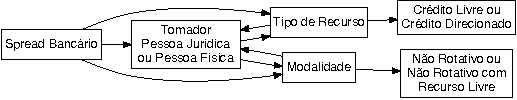
\includegraphics{01-presentation-V1_files/figure-beamer/d.spread.dim-1} \end{center}

\end{frame}

\begin{frame}{\textbf{2.2.2 SPREAD BANCÁRIO NO BRASIL}}
\protect\hypertarget{spread-bancuxe1rio-no-brasil}{}

\begin{itemize}
\item
  Séries mantidas pelo Banco Central:

  \begin{itemize}
  \item
    \emph{Spread} Médio das operações de crédito (MOC)
  \item
    \emph{Spread} do Indicador de Custo de Crédito (ICC)
  \end{itemize}
\item
  Componentes explícitos do \emph{Spread} (BACEN
  \protect\hyperlink{ref-BCB:2000}{2000}):

  \begin{itemize}
  \item
    Inadimplência (\(Ind\))
  \item
    Despesas administrativas (\(DA\))
  \item
    Impostos diretos (\(ID\)) e indiretos (\(II\))
  \item
    Custo de captação (\(CP\))
  \item
    Margem de lucro (\(ML\))
  \end{itemize}
\end{itemize}

\end{frame}

\begin{frame}{\textbf{2.2.2 SPREAD BANCÁRIO NO BRASIL}}
\protect\hypertarget{spread-bancuxe1rio-no-brasil-1}{}

\textbf{DADOS}

\begin{columns}[T]
\begin{column}{0.5\textwidth}
\begin{center}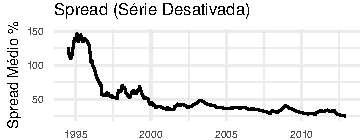
\includegraphics{01-presentation-V1_files/figure-beamer/spread.m.1994.2012-1} \end{center}

\begin{center}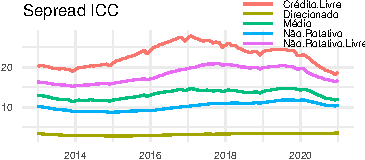
\includegraphics{01-presentation-V1_files/figure-beamer/spread.icc-1} \end{center}
\end{column}

\begin{column}{0.5\textwidth}
\begin{center}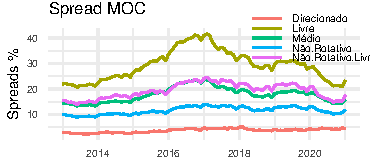
\includegraphics{01-presentation-V1_files/figure-beamer/spread.moct-1} \end{center}

\begin{center}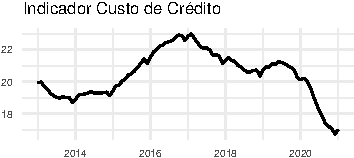
\includegraphics{01-presentation-V1_files/figure-beamer/icc-1} \end{center}
\end{column}
\end{columns}

\end{frame}

\begin{frame}{\textbf{2.2.2 SPREAD BANCÁRIO NO BRASIL}}
\protect\hypertarget{spread-bancuxe1rio-no-brasil-2}{}

\textbf{ESTUDOS EMPÍRICOS}

\begin{itemize}
\item
  Na \textbf{literatura acadêmica} \textbf{não existe} uma
  \textbf{teoria formalizada} acerca do \textbf{\emph{spread}} bancário
  (Magalhães-Timotio \protect\hyperlink{ref-timotio:2018}{2018})
\item
  A \textbf{grande maioria} dos \textbf{estudos} realizados no Brasil
  \textbf{utilizam} as medidas de \textbf{\emph{spread}} bancário
  divulgadas pelo Banco Central, que remetem a uma perspectiva
  \textbf{\emph{ex-ante}} (Dantas
  \protect\hyperlink{ref-dantas:2012}{2012})
\item
  Estudos empíricos \textbf{\emph{spread ex-post}}:

  \begin{itemize}
  \tightlist
  \item
    GUIMARÃES (2002)
  \item
    DANTAS (2012)
  \item
    ALMEIDA (2013)
  \item
    TIMOTIO (2018)
  \end{itemize}
\end{itemize}

\end{frame}

\begin{frame}{\textbf{2.2.2 SPREAD BANCÁRIO NO BRASIL}}
\protect\hypertarget{spread-bancuxe1rio-no-brasil-3}{}

\textbf{VARIÁVEIS IDENTIFICADAS}

\begin{columns}[T]
\begin{column}{0.5\textwidth}
\begin{itemize}
\tightlist
\item
  Modalidade de Instituições
\item
  Controle de Capital
\item
  Relação Crédito/PIB
\item
  Saldo da carteira de crédito
\item
  Indicador do Custo de Crédito
\item
  Selic
\item
  Depósitos Compulsórios
\item
  Despesas Operacionais
\end{itemize}
\end{column}

\begin{column}{0.5\textwidth}
\begin{itemize}
\tightlist
\item
  Inadimplência
\item
  Risco de Crédito
\item
  Dados contábeis padronizadados
\item
  Base Monetária
\item
  Agregados Monetários
\item
  Velocidade da Moeda
\item
  Selic
\item
  Índice HHI - Concentração
\end{itemize}
\end{column}
\end{columns}

\end{frame}

\begin{frame}{\textbf{3. PROCEDIMENTOS METODOLÓGICOS}}
\protect\hypertarget{procedimentos-metodoluxf3gicos}{}

\textbf{FERRAMENTAS}

\begin{itemize}
\item
  Trabalho está sendo desenvolvido e editado em ambiente \textbf{R
  Markdown}
\item
  Utilização de linguagem \textbf{Latex} para padronização de textos,
  figuras e tabelas
\item
  Linguagens \textbf{R} e \textbf{Python} para coleta, tratamento
  modelagem e estimação dos conjuntos de dados.
\item
  Utilizados e construídos \textbf{frameworks}
\end{itemize}

\end{frame}

\begin{frame}{\textbf{3. PROCEDIMENTOS METODOLÓGICOS}}
\protect\hypertarget{procedimentos-metodoluxf3gicos-1}{}

\textbf{DELIMITAÇÃO DOS DADOS}

\begin{itemize}
\item
  Serão selecionadas a ``população'' de instituições bancárias das
  modalidades:

  \begin{itemize}
  \tightlist
  \item
    Banco Múltiplo
  \item
    Banco Comercial
  \item
    Banco de Investimento
  \item
    Banco de Desenvolvimento
  \item
    Caixas Econômicas
  \end{itemize}
\item
  Período entre janeiro 2001 e o outubro de 2020.
\item
  Dados serão obtidos de forma secundária nos bancos de dados abertos do
  Banco Central, IPEA e IBGE e CVM
\end{itemize}

\end{frame}

\begin{frame}{\textbf{3. PROCEDIMENTOS METODOLÓGICOS}}
\protect\hypertarget{procedimentos-metodoluxf3gicos-2}{}

\textbf{PRESSUPOSTOS}

\begin{itemize}
\item
  Será assumido que o \textbf{\emph{spread}} bancário é
  \textbf{definido} diante um conjunto de fatores endógenos e exógenos.
\item
  Assume-se que o \textbf{\emph{spread}} bancário \textbf{não} se
  \textbf{configura} na \textbf{margem de lucro} dos bancos.
\item
  O \textbf{spread} é um dos determinantes de níveis de atividade
  econômica e não o contrário.
\item
  O \textbf{spread} (\(SPR\)) será \textbf{abordado} dentro de uma
  \textbf{concepção} de \textbf{precificação}

  \begin{itemize}
  \tightlist
  \item
    Formado por um conjunto de variáveis explícitas e implícitas
  \end{itemize}
\end{itemize}

\[
Spr = f(E,D,II,DA,ML,IND)
\]

\end{frame}

\begin{frame}{\textbf{3. PROCEDIMENTOS METODOLÓGICOS}}
\protect\hypertarget{procedimentos-metodoluxf3gicos-3}{}

Decomposição partindo da forma tautológica \[
Spr = i_{apl} - i_{cap} 
\] Decomposição da Receita das operações de crédito \[
R = i_{adm}*E + i_{ind}*E + i_{cap}*C + i_{comp}*i_{ac}*C + i_{fgc}*C + \frac{i_{ll}}{1 - i_{r} - i_{cs}}*R + i_{pis}*R + i_{cof}*R 
\] \[
R = E * [i_{adm} + i_{ind} + (\frac{i_{cap}+ i_{fgc} - (i_{comp}*i_{ac})}{1 - i_{comp} - i_{fgc}})] *  \frac{1}
{1 -  \frac{i_{ll}}{1 - i_{ir}  - i_{cs}} - i_{pis} - i_{cof}}
\] - Forma do \emph{Spread} por tipo de capital emprestado
\[\begin{aligned}
& SprEp = [\frac{(D_{pr}* i_{apl})}{E_{pr}} + \frac{(D_{dav}* i_{aplav})}{E_{dav}} + \frac{(D_{dap}* i_{aplap})}{E_{dap}} + ...] - [ \frac{D_{cav}}{C_{av}} + \frac{D_{dap}}{C_{ap}} ]
\end{aligned}\]

\end{frame}

\begin{frame}[fragile]{\textbf{3. PROCEDIMENTOS METODOLÓGICOS}}
\protect\hypertarget{procedimentos-metodoluxf3gicos-4}{}

\textbf{FASE ANALÍTICA}

\begin{itemize}
\tightlist
\item
  Será aplicada a técnica de \textbf{\emph{Cross Validation k-fold}}

  \begin{itemize}
  \item
    Visa \textbf{dividir de forma aleatória o conjunto de dados} em
    \texttt{k} grupos, de dimensão aproximada (James et al.
    \protect\hyperlink{ref-gareth:2017}{2017}).
  \item
    O \textbf{primeiro grupo} é tratado como \textbf{conjunto de
    validação}, e o método é ajustado no \texttt{k\ -\ 1} conjuntos
    restantes (James et al. \protect\hyperlink{ref-gareth:2017}{2017}).
  \item
    Esse \textbf{método} é \textbf{útil} para \textbf{testar variáveis},
    \textbf{selecionar parâmetros}, \textbf{função preditiva} e
    \textbf{acurácia} para \textbf{seleção do modelo final} (James et
    al. \protect\hyperlink{ref-gareth:2017}{2017}).
  \end{itemize}
\item
  Será aplicada a \textbf{técnica de aprendizado não supervisionado
  K-Means}

  \begin{itemize}
  \tightlist
  \item
    \textbf{Particionamento do conjunto de dados} em k
    \textbf{\emph{clusters}} , \textbf{especificados} e \emph{não
    sobrepostos} (James et al.
    \protect\hyperlink{ref-gareth:2017}{2017}).
  \end{itemize}
\end{itemize}

\end{frame}

\begin{frame}{\textbf{3. PROCEDIMENTOS METODOLÓGICOS}}
\protect\hypertarget{procedimentos-metodoluxf3gicos-5}{}

\textbf{MODELO}

\begin{itemize}
\tightlist
\item
  \textbf{Modelo} de \textbf{regressão linear multivariada} (Hill
  \protect\hyperlink{ref-hill:2010}{2010}) (James et al.
  \protect\hyperlink{ref-gareth:2017}{2017}).

  \begin{itemize}
  \tightlist
  \item
    União de técnicas estatísticas e matemáticas para previsão do
    comportamento de uma dada variável dependente, diante um conjunto de
    variáveis explanatórias
  \end{itemize}
\end{itemize}

\[
Y = \beta_0 + \beta_1X_1 + \beta_2X_2...\beta_nX_n + \epsilon
\]

\begin{itemize}
\tightlist
\item
  \textbf{Método} de \emph{dados em painel}, denominado \textbf{Cross
  Section}

  \begin{itemize}
  \tightlist
  \item
    \textbf{\emph{Séries temporais}} e \textbf{\emph{dados em corte
    transversal}}para **captar diferenças individuais de comportamento
    para estimação e inferência (Hill
    \protect\hyperlink{ref-hill:2010}{2010})
  \end{itemize}
\end{itemize}

\begin{enumerate}
[i)]
\tightlist
\item
  Modelo de regressão \textbf{aparentemente não relacionadas (SUR)}
\item
  Modelo de variável binárias (\textbf{efeitos fixos})
\item
  modelo de componentes estocásticos (\textbf{efeitos aleatórios})
\end{enumerate}

\[
y_{it} = \beta_{1it} + \beta_{2it}X_{2it} + \beta_{3it}X_{3it} + e_{it}
\]

\end{frame}

\begin{frame}{\textbf{3. PROCEDIMENTOS METODOLÓGICOS}}
\protect\hypertarget{procedimentos-metodoluxf3gicos-6}{}

\textbf{MODELO 01}

\begin{itemize}
\tightlist
\item
  O \textbf{primeiro modelo} irá verificar a influência das variações de
  variáveis componentes no \textbf{\emph{\emph{Spread Ex-post}}}
\end{itemize}

\textbf{MODELO TEÓRICO} \[\begin{aligned}
SprEp = &f(EPr, EAv, EAp, Atv, ImpInd, ImpId, \\ 
& Inad, MLq, DAdm, Jcp, MSh, HHI, TIns, OCap, \\ 
& CIns, Sel, Ipca, Comp, MPag, VMo, SprEa)
\end{aligned}\]

\textbf{MODELO ECONOMÉTRICO} \[\begin{aligned}
SprEp_{it} = & \beta_{0it} + \beta_{1it}EPr_{it} + \beta_{2it}EAv_{it} + \beta_{3it}EAp_{it} + \beta_{4it}DAdm_{it} + \beta_{5it}Vol_{it} + \\
& \beta_{6it}lnAtv_{it} + \beta_{7it}RC_{it} + \beta_{8it}MSh_{it} + \beta_{9it}HHI_{it} + \\ 
& \beta_{10it}Mod + \beta_{11it}OCap + \beta_{12it}SelOver_{t-1} + \beta_{13it}Ipca_{t-1} + \\
& \beta_{14it}Com_{t} + \beta_{15}Mpag_{t-1} + \beta_{16it}VMo_{t-1} +  \beta_{17t}SprEa_{t-1}
\end{aligned}\]

\end{frame}

\begin{frame}{\textbf{3. PROCEDIMENTOS METODOLÓGICOS}}
\protect\hypertarget{procedimentos-metodoluxf3gicos-7}{}

\textbf{MODELO 02}

\begin{itemize}
\tightlist
\item
  O \textbf{segundo modelo} econométrico testará as variáveis implícitas
  e explícitas com significância estatística do primeiro modelo, atuando
  sobre a rentabilidade bancária \(Rent\)
\end{itemize}

\[\begin{aligned}
Rent_{it} = & \beta_{0it} + \beta_{1it}EPr_{it} + \beta_{2it}EAv_{it} + \beta_{3it}EAp_{it} + \beta_{4it}DAdm_{it} + \beta_{5it}Vol_{it} + \\
& \beta_{6it}lnAtv_{it} + \beta_{7it}RC_{it} + \beta_{8it}MSh_{it} + \beta_{9it}HHI_{it} + \\ 
& \beta_{10it}Mod + \beta_{11it}OCap + \beta_{12it}SelOver_{t-1} + \beta_{13it}Ipca_{t-1} + \\
& \beta_{14it}Com_{t} + \beta_{15}Mpag_{t-1} + \beta_{16it}VMo_{t-1} +  \beta_{17t}SprEa_{t-1}
\end{aligned}\]

\end{frame}

\begin{frame}{\textbf{3. PROCEDIMENTOS METODOLÓGICOS}}
\protect\hypertarget{procedimentos-metodoluxf3gicos-8}{}

\textbf{VARIÁVEIS DEPENDENTES}

\begin{itemize}
\tightlist
\item
  \(SprEp_{it}\): \emph{Spread Ex-post}

  \begin{itemize}
  \tightlist
  \item
    Diferença entre a relação de receitas de operações de crédito
    (\(RcOpCr\)) e operações de crédito média (\(OpCrMe\)) e a Relação
    de despesas de captação (\(DesCap\)) e depósitos médio (\(Dep\)).
  \end{itemize}
\end{itemize}

\[
SprEp_{it} = \frac{RcOpCr_{it}}{\frac{1}{2}(OpCr_{it} + OpCr_{it-1}) } - \frac{DesCap_{it}}{\frac{1}{2}(Dep_{it} + Dep_{it-1})}
\]

\begin{itemize}
\tightlist
\item
  \(Rent\): Relação entre o lucro líquido (\(LLqd\) --- Conta 61800005)
  e as receitas das operações de crédito (\(R\) --- Conta 71100001).
\end{itemize}

\[
Rent_{it} = \frac{LLqd_{it}}{R_{it}}
\]

\end{frame}

\begin{frame}{\textbf{3. PROCEDIMENTOS METODOLÓGICOS}}
\protect\hypertarget{procedimentos-metodoluxf3gicos-9}{}

\textbf{HIPÓTESES}

\begin{longtable}[]{@{}cllcc@{}}
\toprule
Hipótese & Variável & Fórmula & \(SprEp\) & \(Rent\)\tabularnewline
\midrule
\endhead
\(H_{1}\) & (\(EPr\)) &
\(Epr_{it} = \frac{OpCr_{it} - Dep_{it}}{OpCr_{it}}\) & + &
+\tabularnewline
\(H_{2}\) & (\(Eav\)) & \(EAv_{it} = \frac{DepAv_{it}}{OpCr_{it}}\) & +
& +\tabularnewline
\(H_{3}\) & (\(Eap\)) & \(EAp_{it} = \frac{DepAp_{it}}{OpCr_{it}}\) & +
& -\tabularnewline
\(H_{4}\) & (\(DAdm\)) & \(DAdm_{it} = \frac{DA_{it}}{OpCr_{it}}\) & + &
-\tabularnewline
\(H_{5}\) & (\(Vol\)) & \(Vol_{it} = \ln(OpCr_{it})\) & - &
+\tabularnewline
\(H_{6}\) & (\(Tam\)) & \(Tam_{it} = \ln(AtvTot_{it})\) & - &
+\tabularnewline
\bottomrule
\end{longtable}

\end{frame}

\begin{frame}{\textbf{3. PROCEDIMENTOS METODOLÓGICOS}}
\protect\hypertarget{procedimentos-metodoluxf3gicos-10}{}

\textbf{HIPÓTESES}

\begin{longtable}[]{@{}cllcc@{}}
\toprule
\begin{minipage}[b]{0.11\columnwidth}\centering
Hipótese\strut
\end{minipage} & \begin{minipage}[b]{0.15\columnwidth}\raggedright
Variável\strut
\end{minipage} & \begin{minipage}[b]{0.39\columnwidth}\raggedright
Fórmula\strut
\end{minipage} & \begin{minipage}[b]{0.11\columnwidth}\centering
\(SprEp\)\strut
\end{minipage} & \begin{minipage}[b]{0.11\columnwidth}\centering
\(Rent\)\strut
\end{minipage}\tabularnewline
\midrule
\endhead
\begin{minipage}[t]{0.11\columnwidth}\centering
\(H_{7}\)\strut
\end{minipage} & \begin{minipage}[t]{0.15\columnwidth}\raggedright
(\(RC\))\strut
\end{minipage} & \begin{minipage}[t]{0.39\columnwidth}\raggedright
\(T_{RCit} = \frac{\frac{\sum_{RC = Aa}^HOC_{RC}*P_{RC}}{\sum_{}P_{RC}}}{\sum_{OC_{RC}}}\)\strut
\end{minipage} & \begin{minipage}[t]{0.11\columnwidth}\centering
+\strut
\end{minipage} & \begin{minipage}[t]{0.11\columnwidth}\centering
+\strut
\end{minipage}\tabularnewline
\begin{minipage}[t]{0.11\columnwidth}\centering
\(H_{8}\)\strut
\end{minipage} & \begin{minipage}[t]{0.15\columnwidth}\raggedright
(\(MkSh\))\strut
\end{minipage} & \begin{minipage}[t]{0.39\columnwidth}\raggedright
\(MkSh_{it} = \frac{OpCr_{it}}{\sum_{t=1}^nOpCr_{it}}\)\strut
\end{minipage} & \begin{minipage}[t]{0.11\columnwidth}\centering
-\strut
\end{minipage} & \begin{minipage}[t]{0.11\columnwidth}\centering
+\strut
\end{minipage}\tabularnewline
\begin{minipage}[t]{0.11\columnwidth}\centering
\(H_{9}\)\strut
\end{minipage} & \begin{minipage}[t]{0.15\columnwidth}\raggedright
(\(GC\))\strut
\end{minipage} & \begin{minipage}[t]{0.39\columnwidth}\raggedright
\(HHI_{it} = \frac{1}{n} + n\frac{\sum_{i=1}^{n}(\frac{R_{it} - 1}{n})^2}{n}\)\strut
\end{minipage} & \begin{minipage}[t]{0.11\columnwidth}\centering
+\strut
\end{minipage} & \begin{minipage}[t]{0.11\columnwidth}\centering
+\strut
\end{minipage}\tabularnewline
\begin{minipage}[t]{0.11\columnwidth}\centering
\(H_{10}\)\strut
\end{minipage} & \begin{minipage}[t]{0.15\columnwidth}\raggedright
(\(Mod\))\strut
\end{minipage} & \begin{minipage}[t]{0.39\columnwidth}\raggedright
\(D_{1}...D_{5}\)\strut
\end{minipage} & \begin{minipage}[t]{0.11\columnwidth}\centering
\emph{dummy}\strut
\end{minipage} & \begin{minipage}[t]{0.11\columnwidth}\centering
\emph{dummy}\strut
\end{minipage}\tabularnewline
\begin{minipage}[t]{0.11\columnwidth}\centering
\(H_{11}\)\strut
\end{minipage} & \begin{minipage}[t]{0.15\columnwidth}\raggedright
(\(OCap\))\strut
\end{minipage} & \begin{minipage}[t]{0.39\columnwidth}\raggedright
\(D_{6}...D_{10}\)\strut
\end{minipage} & \begin{minipage}[t]{0.11\columnwidth}\centering
\emph{dummy}\strut
\end{minipage} & \begin{minipage}[t]{0.11\columnwidth}\centering
\emph{dummy}\strut
\end{minipage}\tabularnewline
\begin{minipage}[t]{0.11\columnwidth}\centering
\(H_{12}\)\strut
\end{minipage} & \begin{minipage}[t]{0.15\columnwidth}\raggedright
\(SelOver\)\strut
\end{minipage} & \begin{minipage}[t]{0.39\columnwidth}\raggedright
\(Sel_{t-1} = \frac{1}{n}\sum_{t=-1}^{n-1}SelDrAn\)\strut
\end{minipage} & \begin{minipage}[t]{0.11\columnwidth}\centering
+\strut
\end{minipage} & \begin{minipage}[t]{0.11\columnwidth}\centering
+\strut
\end{minipage}\tabularnewline
\bottomrule
\end{longtable}

\end{frame}

\begin{frame}{\textbf{3. PROCEDIMENTOS METODOLÓGICOS}}
\protect\hypertarget{procedimentos-metodoluxf3gicos-11}{}

\textbf{HIPÓTESES}

\begin{longtable}[]{@{}cllcc@{}}
\toprule
\begin{minipage}[b]{0.11\columnwidth}\centering
Hipótese\strut
\end{minipage} & \begin{minipage}[b]{0.15\columnwidth}\raggedright
Variável\strut
\end{minipage} & \begin{minipage}[b]{0.39\columnwidth}\raggedright
Fórmula\strut
\end{minipage} & \begin{minipage}[b]{0.11\columnwidth}\centering
\(SprEp\)\strut
\end{minipage} & \begin{minipage}[b]{0.11\columnwidth}\centering
\(Rent\)\strut
\end{minipage}\tabularnewline
\midrule
\endhead
\begin{minipage}[t]{0.11\columnwidth}\centering
\(H_{13}\)\strut
\end{minipage} & \begin{minipage}[t]{0.15\columnwidth}\raggedright
(\(Ipca\))\strut
\end{minipage} & \begin{minipage}[t]{0.39\columnwidth}\raggedright
\(Ipca_{t-1} = \frac{1}{n}\sum_{t=-1}^{n-1}IpcaMs\)\strut
\end{minipage} & \begin{minipage}[t]{0.11\columnwidth}\centering
+\strut
\end{minipage} & \begin{minipage}[t]{0.11\columnwidth}\centering
-\strut
\end{minipage}\tabularnewline
\begin{minipage}[t]{0.11\columnwidth}\centering
\(H_{14}\)\strut
\end{minipage} & \begin{minipage}[t]{0.15\columnwidth}\raggedright
(\(Com\))\strut
\end{minipage} & \begin{minipage}[t]{0.39\columnwidth}\raggedright
\(Comp_{t} = \frac{RcDAv_{t} + RcDAp_{t}}{\sum_{t=1}^{n}DAv_{it} + \sum_{t=1}^{n}DAp_{it}}\)\strut
\end{minipage} & \begin{minipage}[t]{0.11\columnwidth}\centering
+\strut
\end{minipage} & \begin{minipage}[t]{0.11\columnwidth}\centering
-\strut
\end{minipage}\tabularnewline
\begin{minipage}[t]{0.11\columnwidth}\centering
\(H_{15}\)\strut
\end{minipage} & \begin{minipage}[t]{0.15\columnwidth}\raggedright
\(Mpag\)\strut
\end{minipage} & \begin{minipage}[t]{0.39\columnwidth}\raggedright
\(Mapg_{t} = \ln(MPM4_{t-1})\)\strut
\end{minipage} & \begin{minipage}[t]{0.11\columnwidth}\centering
-\strut
\end{minipage} & \begin{minipage}[t]{0.11\columnwidth}\centering
+\strut
\end{minipage}\tabularnewline
\begin{minipage}[t]{0.11\columnwidth}\centering
\(H_{16}\)\strut
\end{minipage} & \begin{minipage}[t]{0.15\columnwidth}\raggedright
(\(VelMo\))\strut
\end{minipage} & \begin{minipage}[t]{0.39\columnwidth}\raggedright
\(VelMo_{t} = \frac{Pib_{t-1}}{BMr_{t-1}}\)\strut
\end{minipage} & \begin{minipage}[t]{0.11\columnwidth}\centering
-\strut
\end{minipage} & \begin{minipage}[t]{0.11\columnwidth}\centering
+\strut
\end{minipage}\tabularnewline
\begin{minipage}[t]{0.11\columnwidth}\centering
\(H_{17}\)\strut
\end{minipage} & \begin{minipage}[t]{0.15\columnwidth}\raggedright
(\(SprEa_{t-1}\))\strut
\end{minipage} & \begin{minipage}[t]{0.39\columnwidth}\raggedright
\(SprEa_{t} = SEA_{t-1}\)\strut
\end{minipage} & \begin{minipage}[t]{0.11\columnwidth}\centering
+\strut
\end{minipage} & \begin{minipage}[t]{0.11\columnwidth}\centering
+\strut
\end{minipage}\tabularnewline
\bottomrule
\end{longtable}

\end{frame}

\begin{frame}{\textbf{3. PROCEDIMENTOS METODOLÓGICOS}}
\protect\hypertarget{procedimentos-metodoluxf3gicos-12}{}

\textbf{RESUMO DE DADOS}

\begin{longtable}[]{@{}llll@{}}
\toprule
\textbf{Nome} & \textbf{Código} & \textbf{Periodicidade} &
\textbf{Fonte}\tabularnewline
\midrule
\endhead
Dados Financeiros & 370 & Mensal & Banco Central\tabularnewline
PIB & BM12\_PIB12 & Mensal & IPEA\tabularnewline
Selic Over & BM12\_TJOVER12 & Mensal & Banco Central\tabularnewline
Meios de Pagamentos & BM12\_M4NCN12 & Mensal & IPEA\tabularnewline
IPCA & PRECOS12\_IPCAG12 & Mensal & IPEA\tabularnewline
Compulsório Poupança & 1848 & Mensal & Banco Central\tabularnewline
Compulsório a vista & 1849 & Mensal & Banco Central\tabularnewline
Compulsório a prazo & 1850 & Mensal & Banco Central\tabularnewline
Base Monetária Ampliada & 1833 & Mensal & Banco Central\tabularnewline
\bottomrule
\end{longtable}

\end{frame}

\begin{frame}{\textbf{REFERÊNCIAS}}
\protect\hypertarget{referuxeancias}{}

BACEN. 2000. ``Juros E Spread Bancário No Brasil.'' Brasília: Banco
Central do Brasil.
\url{https://www.bcb.gov.br/ftp/jurospread112000.pdf}.

---------. 2016. ``Juros E Spread Bancário.'' Brasília: Banco Central do
Brasil. BANK, WORLD, and IMF. 2005. Financial Sector Assessment: A
Handbook. Washington DCo: The World Bank.
\url{http://documents1.worldbank.org/curated/en/306701468337879923/pdf/}
337970rev0Fina10Assessment01PUBLIC1.pdf.

Dantas, José A. 2012. ``Determinantes Do Spread Bancário Ex Post No
Mercado Brasileiro.'' REV. ADM. MACKENZIE 13 (4). UNIVERSIDADE
PRESBITERIANA MACKENZIE: 48--74.

\end{frame}

\begin{frame}{\textbf{REFERÊNCIAS}}
\protect\hypertarget{referuxeancias-1}{}

Dick, Astrid. 1999. ``Banking Spreads in Central America: Evolution,
Structure, and Behavior.'' HIID Development Discussion Papers. Harvard
Institute for International Development, Cambridge.

Hill, R. Carter. 2010. Economertia. 3rd ed. São Paulo: Saraiva.

Gareth, 2017. An Introduction to Statistical Learning. 8th ed. New York:
Springer.

Leal, Rodrigo Mendes. 2006. ``Estrutura E Determinantes Do Spread
Bancário No Brasil:Uma Resenha Comparativa Da Literatura Empírica.'' Rio
de Janeiro: Universidade do Estado do Rio de Janeiro.

\end{frame}

\begin{frame}{\textbf{REFERÊNCIAS}}
\protect\hypertarget{referuxeancias-2}{}

Levine, Ross. 1997. ``Financial Development and Economic Growth: Views
and Agenda.'' Journal of Economic Literature 35 (2). American Economic
Association: 688--726. \url{http://www.jstor.org/stable/2729790}.

Magalhães-Timotio, João G. 2018. ``Relação entre Indicadores Contábeis E
O Spread Ex-Post Dos Bancos Brasileiros.'' RACEF -- Revista de
Administração, Contabilidade E Economia Da Fundace 9 (2): 31--44.

Matos, Orlando Carneiro de. 2003. ``Inter-Relações Entre Desenvolvimento
Financeiro, Exportações E Crescimento Econômico: Análise Da Experiênncia
Brasileira.''

\end{frame}

\begin{frame}{\textbf{AGRADECIMENTOS}}
\protect\hypertarget{agradecimentos}{}

\textbf{OBRIGADO}

\end{frame}

\begin{frame}{\textbf{REFERÊNCIAS}}
\protect\hypertarget{referuxeancias-3}{}

\hypertarget{refs}{}
\leavevmode\hypertarget{ref-BCB:2000}{}%
BACEN. 2000. ``Juros E Spread Bancário No Brasil.'' Brasília: Banco
Central do Brasil.
\url{https://www.bcb.gov.br/ftp/jurospread112000.pdf}.

\leavevmode\hypertarget{ref-BCB:2016}{}%
---------. 2016. ``Juros E Spread Bancário.'' Brasília: Banco Central do
Brasil.

\leavevmode\hypertarget{ref-WB:2005}{}%
BANK, WORLD, and IMF. 2005. \emph{Financial Sector Assessment: A
Handbook}. Washington DCo: The World Bank.
\url{http://documents1.worldbank.org/curated/en/306701468337879923/pdf/337970rev0Fina10Assessment01PUBLIC1.pdf}.

\leavevmode\hypertarget{ref-dantas:2012}{}%
Dantas, José A. 2012. ``Determinantes Do Spread Bancário Ex Post No
Mercado Brasileiro.'' \emph{REV. ADM. MACKENZIE} 13 (4). UNIVERSIDADE
PRESBITERIANA MACKENZIE: 48--74.

\leavevmode\hypertarget{ref-dick:1999}{}%
Dick, Astrid. 1999. ``Banking Spreads in Central America: Evolution,
Structure, and Behavior.'' \emph{HIID Development Discussion Papers}.
Harvard Institute for International Development, Cambridge.

\leavevmode\hypertarget{ref-hill:2010}{}%
Hill, R. Carter. 2010. \emph{Economertia}. 3rd ed. São Paulo: Saraiva.

\leavevmode\hypertarget{ref-gareth:2017}{}%
James, Gareth, Daniela Witten, Trevor Hastie, and Robert Tibshirani.
2017. \emph{An Introduction to Statistical Learning}. 8th ed. New York:
Springer.

\leavevmode\hypertarget{ref-leal:2006}{}%
Leal, Rodrigo Mendes. 2006. ``Estrutura E Determinantes Do Spread
Bancário No Brasil:Uma Resenha Comparativa Da Literatura Empírica.'' Rio
de Janeiro: Universidade do Estado do Rio de Janeiro.

\leavevmode\hypertarget{ref-levine:1997}{}%
Levine, Ross. 1997. ``Financial Development and Economic Growth: Views
and Agenda.'' \emph{Journal of Economic Literature} 35 (2). American
Economic Association: 688--726.
\url{http://www.jstor.org/stable/2729790}.

\leavevmode\hypertarget{ref-timotio:2018}{}%
Magalhães-Timotio, João G. 2018. ``RELAÇÃO Entre Indicadores Contábeis E
O Spread Ex-Post Dos Bancos Brasileiros.'' \emph{RACEF -- Revista de
Administração, Contabilidade E Economia Da Fundace} 9 (2): 31--44.

\leavevmode\hypertarget{ref-matos:2003}{}%
Matos, Orlando Carneiro de. 2003. ``Inter-Relações Entre Desenvolvimento
Financeiro, Exportações E Crescimento Econômico: Análise Da Experiência
Brasileira.'' In \emph{Notas Técnicas Do Banco Central Do Brasil}.
Brasília: BCB.
\url{https://www.bcb.gov.br/content/publicacoes/notastecnicas/2003nt40Inter-relentreDesenvFinanp.pdf}.

\end{frame}

\end{document}
